% Note that the a4paper option is mainly intended so that authors in
% countries using A4 can easily print to A4 and see how their papers will
% look in print - the typesetting of the document will not typically be
% affected with changes in paper size (but the bottom and side margins will).
% Use the testflow package mentioned above to verify correct handling of
% both paper sizes by the user's LaTeX system.
%
% Also note that the "draftcls" or "draftclsnofoot", not "draft", option
% should be used if it is desired that the figures are to be displayed in
% draft mode.
%
\documentclass[conference]{IEEEtran}
% Add the compsoc option for Computer Society conferences.
%
% If IEEEtran.cls has not been installed into the LaTeX system files,
% manually specify the path to it like:
% \documentclass[conference]{../sty/IEEEtran}





% Some very useful LaTeX packages include:
% (uncomment the ones you want to load)


% *** MISC UTILITY PACKAGES ***
%
%\usepackage{ifpdf}
% Heiko Oberdiek's ifpdf.sty is very useful if you need conditional
% compilation based on whether the output is pdf or dvi.
% usage:
% \ifpdf
%   % pdf code
% \else
%   % dvi code
% \fi
% The latest version of ifpdf.sty can be obtained from:
% http://www.ctan.org/tex-archive/macros/latex/contrib/oberdiek/
% Also, note that IEEEtran.cls V1.7 and later provides a builtin
% \ifCLASSINFOpdf conditional that works the same way.
% When switching from latex to pdflatex and vice-versa, the compiler may
% have to be run twice to clear warning/error messages.






% *** CITATION PACKAGES ***
%
%\usepackage{cite}
% cite.sty was written by Donald Arseneau
% V1.6 and later of IEEEtran pre-defines the format of the cite.sty package
% \cite{} output to follow that of IEEE. Loading the cite package will
% result in citation numbers being automatically sorted and properly
% "compressed/ranged". e.g., [1], [9], [2], [7], [5], [6] without using
% cite.sty will become [1], [2], [5]--[7], [9] using cite.sty. cite.sty's
% \cite will automatically add leading space, if needed. Use cite.sty's
% noadjust option (cite.sty V3.8 and later) if you want to turn this off.
% cite.sty is already installed on most LaTeX systems. Be sure and use
% version 4.0 (2003-05-27) and later if using hyperref.sty. cite.sty does
% not currently provide for hyperlinked citations.
% The latest version can be obtained at:
% http://www.ctan.org/tex-archive/macros/latex/contrib/cite/
% The documentation is contained in the cite.sty file itself.






% *** GRAPHICS RELATED PACKAGES ***
%
\ifCLASSINFOpdf
  \usepackage[pdftex]{graphicx}
  % declare the path(s) where your graphic files are
  % \graphicspath{{../pdf/}{../jpeg/}}
  % and their extensions so you won't have to specify these with
  % every instance of \includegraphics
  \DeclareGraphicsExtensions{.pdf,.jpeg,.png}
\else
  % or other class option (dvipsone, dvipdf, if not using dvips). graphicx
  % will default to the driver specified in the system graphics.cfg if no
  % driver is specified.
  % \usepackage[dvips]{graphicx}
  % declare the path(s) where your graphic files are
  % \graphicspath{{../eps/}}
  % and their extensions so you won't have to specify these with
  % every instance of \includegraphics
  % \DeclareGraphicsExtensions{.eps}
\fi
% graphicx was written by David Carlisle and Sebastian Rahtz. It is
% required if you want graphics, photos, etc. graphicx.sty is already
% installed on most LaTeX systems. The latest version and documentation can
% be obtained at: 
% http://www.ctan.org/tex-archive/macros/latex/required/graphics/
% Another good source of documentation is "Using Imported Graphics in
% LaTeX2e" by Keith Reckdahl which can be found as epslatex.ps or
% epslatex.pdf at: http://www.ctan.org/tex-archive/info/
%
% latex, and pdflatex in dvi mode, support graphics in encapsulated
% postscript (.eps) format. pdflatex in pdf mode supports graphics
% in .pdf, .jpeg, .png and .mps (metapost) formats. Users should ensure
% that all non-photo figures use a vector format (.eps, .pdf, .mps) and
% not a bitmapped formats (.jpeg, .png). IEEE frowns on bitmapped formats
% which can result in "jaggedy"/blurry rendering of lines and letters as
% well as large increases in file sizes.
%
% You can find documentation about the pdfTeX application at:
% http://www.tug.org/applications/pdftex





% *** MATH PACKAGES ***
%
%\usepackage[cmex10]{amsmath}
% A popular package from the American Mathematical Society that provides
% many useful and powerful commands for dealing with mathematics. If using
% it, be sure to load this package with the cmex10 option to ensure that
% only type 1 fonts will utilized at all point sizes. Without this option,
% it is possible that some math symbols, particularly those within
% footnotes, will be rendered in bitmap form which will result in a
% document that can not be IEEE Xplore compliant!
%
% Also, note that the amsmath package sets \interdisplaylinepenalty to 10000
% thus preventing page breaks from occurring within multiline equations. Use:
%\interdisplaylinepenalty=2500
% after loading amsmath to restore such page breaks as IEEEtran.cls normally
% does. amsmath.sty is already installed on most LaTeX systems. The latest
% version and documentation can be obtained at:
% http://www.ctan.org/tex-archive/macros/latex/required/amslatex/math/





% *** SPECIALIZED LIST PACKAGES ***
%
%\usepackage{algorithmic}
% algorithmic.sty was written by Peter Williams and Rogerio Brito.
% This package provides an algorithmic environment fo describing algorithms.
% You can use the algorithmic environment in-text or within a figure
% environment to provide for a floating algorithm. Do NOT use the algorithm
% floating environment provided by algorithm.sty (by the same authors) or
% algorithm2e.sty (by Christophe Fiorio) as IEEE does not use dedicated
% algorithm float types and packages that provide these will not provide
% correct IEEE style captions. The latest version and documentation of
% algorithmic.sty can be obtained at:
% http://www.ctan.org/tex-archive/macros/latex/contrib/algorithms/
% There is also a support site at:
% http://algorithms.berlios.de/index.html
% Also of interest may be the (relatively newer and more customizable)
% algorithmicx.sty package by Szasz Janos:
% http://www.ctan.org/tex-archive/macros/latex/contrib/algorithmicx/




% *** ALIGNMENT PACKAGES ***
%
\usepackage{array}
% Frank Mittelbach's and David Carlisle's array.sty patches and improves
% the standard LaTeX2e array and tabular environments to provide better
% appearance and additional user controls. As the default LaTeX2e table
% generation code is lacking to the point of almost being broken with
% respect to the quality of the end results, all users are strongly
% advised to use an enhanced (at the very least that provided by array.sty)
% set of table tools. array.sty is already installed on most systems. The
% latest version and documentation can be obtained at:
% http://www.ctan.org/tex-archive/macros/latex/required/tools/


%\usepackage{mdwmath}
%\usepackage{mdwtab}
% Also highly recommended is Mark Wooding's extremely powerful MDW tools,
% especially mdwmath.sty and mdwtab.sty which are used to format equations
% and tables, respectively. The MDWtools set is already installed on most
% LaTeX systems. The lastest version and documentation is available at:
% http://www.ctan.org/tex-archive/macros/latex/contrib/mdwtools/


% IEEEtran contains the IEEEeqnarray family of commands that can be used to
% generate multiline equations as well as matrices, tables, etc., of high
% quality.


%\usepackage{eqparbox}
% Also of notable interest is Scott Pakin's eqparbox package for creating
% (automatically sized) equal width boxes - aka "natural width parboxes".
% Available at:
% http://www.ctan.org/tex-archive/macros/latex/contrib/eqparbox/





% *** SUBFIGURE PACKAGES ***
\usepackage[tight,footnotesize]{subfigure}
% subfigure.sty was written by Steven Douglas Cochran. This package makes it
% easy to put subfigures in your figures. e.g., "Figure 1a and 1b". For IEEE
% work, it is a good idea to load it with the tight package option to reduce
% the amount of white space around the subfigures. subfigure.sty is already
% installed on most LaTeX systems. The latest version and documentation can
% be obtained at:
% http://www.ctan.org/tex-archive/obsolete/macros/latex/contrib/subfigure/
% subfigure.sty has been superceeded by subfig.sty.



%\usepackage[caption=false]{caption}
%\usepackage[font=footnotesize]{subfig}
% subfig.sty, also written by Steven Douglas Cochran, is the modern
% replacement for subfigure.sty. However, subfig.sty requires and
% automatically loads Axel Sommerfeldt's caption.sty which will override
% IEEEtran.cls handling of captions and this will result in nonIEEE style
% figure/table captions. To prevent this problem, be sure and preload
% caption.sty with its "caption=false" package option. This is will preserve
% IEEEtran.cls handing of captions. Version 1.3 (2005/06/28) and later 
% (recommended due to many improvements over 1.2) of subfig.sty supports
% the caption=false option directly:
%\usepackage[caption=false,font=footnotesize]{subfig}
%
% The latest version and documentation can be obtained at:
% http://www.ctan.org/tex-archive/macros/latex/contrib/subfig/
% The latest version and documentation of caption.sty can be obtained at:
% http://www.ctan.org/tex-archive/macros/latex/contrib/caption/




% *** FLOAT PACKAGES ***
%
%\usepackage{fixltx2e}
% fixltx2e, the successor to the earlier fix2col.sty, was written by
% Frank Mittelbach and David Carlisle. This package corrects a few problems
% in the LaTeX2e kernel, the most notable of which is that in current
% LaTeX2e releases, the ordering of single and double column floats is not
% guaranteed to be preserved. Thus, an unpatched LaTeX2e can allow a
% single column figure to be placed prior to an earlier double column
% figure. The latest version and documentation can be found at:
% http://www.ctan.org/tex-archive/macros/latex/base/



%\usepackage{stfloats}
% stfloats.sty was written by Sigitas Tolusis. This package gives LaTeX2e
% the ability to do double column floats at the bottom of the page as well
% as the top. (e.g., "\begin{figure*}[!b]" is not normally possible in
% LaTeX2e). It also provides a command:
%\fnbelowfloat
% to enable the placement of footnotes below bottom floats (the standard
% LaTeX2e kernel puts them above bottom floats). This is an invasive package
% which rewrites many portions of the LaTeX2e float routines. It may not work
% with other packages that modify the LaTeX2e float routines. The latest
% version and documentation can be obtained at:
% http://www.ctan.org/tex-archive/macros/latex/contrib/sttools/
% Documentation is contained in the stfloats.sty comments as well as in the
% presfull.pdf file. Do not use the stfloats baselinefloat ability as IEEE
% does not allow \baselineskip to stretch. Authors submitting work to the
% IEEE should note that IEEE rarely uses double column equations and
% that authors should try to avoid such use. Do not be tempted to use the
% cuted.sty or midfloat.sty packages (also by Sigitas Tolusis) as IEEE does
% not format its papers in such ways.





% *** PDF, URL AND HYPERLINK PACKAGES ***
%
%\usepackage{url}
% url.sty was written by Donald Arseneau. It provides better support for
% handling and breaking URLs. url.sty is already installed on most LaTeX
% systems. The latest version can be obtained at:
% http://www.ctan.org/tex-archive/macros/latex/contrib/misc/
% Read the url.sty source comments for usage information. Basically,
% \url{my_url_here}.





% *** Do not adjust lengths that control margins, column widths, etc. ***
% *** Do not use packages that alter fonts (such as pslatex).         ***
% There should be no need to do such things with IEEEtran.cls V1.6 and later.
% (Unless specifically asked to do so by the journal or conference you plan
% to submit to, of course. )


% correct bad hyphenation here
\hyphenation{op-tical net-works semi-conduc-tor}


\begin{document}
%
% paper title
% can use linebreaks \\ within to get better formatting as desired
\title{Shape recognition under various noise conditions using smoothed Harris corner detector}


% author names and affiliations
% use a multiple column layout for up to three different
% affiliations
\author{\IEEEauthorblockN{Michael Single}
\IEEEauthorblockA{University of Berne\\
08-917-445}
\and
\IEEEauthorblockN{Stefan Moser}
\IEEEauthorblockA{University of Berne\\
09-277-013}
}


% make the title area
\maketitle


\begin{abstract}
%\boldmath
We are using a Harris corner detector\cite{Harris88acombined} 
to classify simple geometric shapes. Further, we 
investigated on the impact of various types of noise on the classification and ways
to preprocess the distorted images to improve classification results.
\end{abstract}

\section{Introduction}
% no \IEEEPARstart
Shape recognition has been an interest in computer science since long ago. Especially in the
field of text recognition there is the task to classify scanned characters to construct 
a digital representation of a text.

\section{Algorithm}
The goal of our algorithm is to detect the type of shape contained in a provided binary valued image. 
Such a given image may suffer from either different types of noise or its shapes may exhibit fringes. \\

% TODO: ADD FIGURE Depicting IMAGE OF SHAPE TYPES and their possible degenerations degeneration

In this work we only are interested in detecting triangle-, square-, regular 5-star- or circle-shapes. However, each such shape can be arbitrary oriented and scaled. \\

The key idea of our approach is to detect all corners of a shape-image and then classify a shape according to the detected numbers of corners. For this purpose we decided to implement a Harris corner detector. Such a detector works well for clean images (FOOTNOTE: i.e. images that do not suffer from noise or exhibit shapes having fringes). However, since given images may suffer from various degenerations, a preprocessing of the input is required before applying the classification. \\

In summary our algorithm does the following for each given input image:
	\begin{itemize}
		\item Detect type of degeneration present in input image
		\item Apply corresponding preprocessing step
		\item Detect Corners and Classify
	\end{itemize}  
	
In the following a more detailed explanation how the separate algorithmic steps work.

\subsection{Detect Degeneration Type}
Given input images may suffer from either noise or the edges of the shapes could be fringed.
Hence, we first want to detect the type of image degeneration and then apply a customized preprocessing that directly addresses present issue. Our algorithm is able to detect whether an image exhibits Gaussian noise, salt-and-pepper noise, fringes shape edges or has no (significant) degeneration. \\

Since our image is binary valued we can detect Gaussian noise by computing the histogram of the image. If it has more than two bins (zero/one-valued bins) then we know there are other responses present in the image which is a characteristic property of Gaussian noise. \\

The salt-and-pepper noise can be detected (and also corrected) by applying a median filter onto an image. 
Therefore we simply apply a median filter with window size of 5x5 pixels onto the image and compute the difference between the input image and its median filtered version. 
In case the difference is too large we assume that there is salt-and-pepper noise present. \\

Finally, we need to detect jagged edges on the input (dents and bulges along edges, see Figure \ref{fig:triangle_fringes} for an example). 
Throughout this report we call this type of distortion \emph{fringes}. 
Here, we extract the difference between a clean version of the image and the fringe version by computing some border along the fringe image. 
If the difference is too big, we say there are fringes present. \\
	
Technically, we apply a blur-kernel onto the image. Then, we compute a mask by applying a thresholding. Each blurred pixel value that is too small is set to zero and otherwise its value is assigned to one. We combine this mask with the input image by a component-wise operation. The result is a binary image with pixels equal one if the other images were one too at that pixel location and otherwise is zero. We count all pixels equal one and decide whether this corresponds to a fringe count.
	
	
	% TODO (ADD FOOTNOTE: in our convention one means that the pixel belongs to the shape and zero that the pixel belongs to the background. 

If none of the previously described checks yielded a positive result, we assume that our image does not suffer from any kind of degeneration.
  
\subsection{Preprocessing}
From the degeneration detection step we know what kind of issues we have to deal with. The simplest case occurs if no noise has been detected. Then our algorithm can skip this step and thus can directly start to detect corners in the image. \\

When fringes have been detected we need to restore the edges.
The idea is to smooth the edges out and then compute a new binary image simple thresholding. 
For smoothing, we use a bilinear filter\cite{TomasiBilateralFiltering}, since we want mainly smoothing along edges, but not blur the edge itself. A more detailed motivation behind this
choice can be seen in Figure \ref{fig:bilateral_vs_gaussian_smoothed}. \\

In case salt-and-pepper noise was detected, we have to apply a so called median filter. Such a filter performs a salt-and-pepper noise reduction by removing outlier peak responses in the input image. Technically, this is achieved by convolving the input image with local neighbourhood-window that got its center value replaced with its median value. However, the filtered image suffers now from some kind of soft-fringes. this is why we also have to apply the edge restoration step described above before. \\

For Gaussian noise assume we have given a degradation model where noise behaves additively and is normal distributed. Using such a noise-model we are allowed to apply so called Wiener-Filter (a non-linear probabilistic noise reduction). 

\subsection{Corner Detection}
\label{sub:corner_detection}
Given a pre-processed clean image of a shape we want to find its corners. Our constraint that each image only contains one shape allows us to directly relate the number of detected corners with the type of shape we are dealing with. \\

For detecting corners we rely on the so called Harris corner detector. We can think of it as a special kind of kernel applied to the image. the result is a binary image that only exhibits some small pixel blobs, usually having a radius at most of 3 pixels. These blobs are supposed to form the corners of the image. \\ 

In general, a corner can be interpreted as a point in the image that has two dominant and different edge directions in its local neighbourhood. The goal of the Harris corner detector is to find those points. \\

Edges in an image are points that depict some form of rapid change of pixel intensity. In other words an edge is a series of locale maximal values. A maxima corresponds to either the smallest or the largest derivate within a given domain. Since either a minimum or a maximum depict a valid potential edge, we simply can compute the image gradient and take its absolute value. The gradient of a 2d image is a vector field containing two components, i.e. each pixel in the image is mapped to a vector. The first component is the derivative along the x-direction, the 2nd is the derivate along the y-direction. We interpret the absolute value as the 2-norm in the image. \\

In oder to only detect strong maxima, a Harris filter also makes use of the product of the two single derivate directions. This can be interpreted as some kind of weighting that ensures that we only consider strong edge-intensities. \\

In order to make the Harris filter more robust, one does usually have to apply a pre-smoothing onto the image. This also ensures to smooth-out small peaks in the image that would be vanish due to the taking derivative step. \\

Mathematically, the harris kernel looks like the following: 

The Eigenvalues of the filtered images tell us whether we are dealing with a corner, an edge or a non-existing feature. If the two largest eigenvalues both are sufficiently large we have detected a corner.

\subsection{Shape Classification}
The classification of a shape is actually the simplest processing step. We simply the number of detected corners resulting from the previous step. There is a one to one correspondence between the number of detected corners and the number of corners that a triangular or squared shape exhibit. However, when given a circular shape, our Harris detector does return zero corners. Thus, if we have zero corners detected, we assume we found a circle. Lastly, there is the classification of the 5-star. Most of the times our Harris detector is robust enough and detects 5 corners. However, there are certain cases when it detects more than 5 corners. Therefore we assume we detected a 5-star shape if the corner count is at least equal 5.


\begin{figure}%
\centering
\subfigure[Shape]{
\includegraphics[width=0.1\textwidth]{square}}
\subfigure[Response]{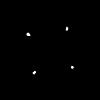
\includegraphics[width=0.1\textwidth]{square_response}}\\
\subfigure[Sx]{
\includegraphics[width=0.1\textwidth]{square_sx2_smoothed}}
\subfigure[Sy]{
\includegraphics[width=0.1\textwidth]{square_sy2_smoothed}}
\subfigure[Sxy]{
\includegraphics[width=0.1\textwidth]{square_sxy_smoothed}}
\caption{A square and TODO}

\end{figure}

\begin{figure}%
\centering
\subfigure[Triangle with fringes.]{
\includegraphics[width=0.1\textwidth]{triangle_noisy} \label{fig:triangle_fringes}}
\subfigure[Preprocessed]{
\includegraphics[width=0.1\textwidth]{triangle_noisy_preprocessed}} \\
\subfigure[Response]{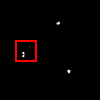
\includegraphics[width=0.1\textwidth]{triangle_noisy_response_with_rect}}
\subfigure[Detail of response]{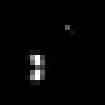
\includegraphics[width=0.1\textwidth]{triangle_noisy_detail_response}}
\caption{Nasty double peak and tiny thingy}

\end{figure}% subsection corner_detection (end)

\section{Results}

For images without noise we achieve a recognition rate of 100\%. 

\section{Conclusion}
% TODO write mini summary
% TODO mention that our detector is also able to detect Gaussian noise
% mention draw-backs and adv. 
% mention other ideas and directions

\label{sec:results}

% section results (end)
% An example of a floating figure using the graphicx package.
% Note that \label must occur AFTER (or within) \caption.
% For figures, \caption should occur after the \includegraphics.
% Note that IEEEtran v1.7 and later has special internal code that
% is designed to preserve the operation of \label within \caption
% even when the captionsoff option is in effect. However, because
% of issues like this, it may be the safest practice to put all your
% \label just after \caption rather than within \caption{}.
%
% Reminder: the "draftcls" or "draftclsnofoot", not "draft", class
% option should be used if it is desired that the figures are to be
% displayed while in draft mode.
%
%\begin{figure}[!t]
%\centering
%\includegraphics[width=2.5in]{myfigure}
% where an .eps filename suffix will be assumed under latex, 
% and a .pdf suffix will be assumed for pdflatex; or what has been declared
% via \DeclareGraphicsExtensions.
%\caption{Simulation Results}
%\label{fig_sim}
%\end{figure}

% Note that IEEE typically puts floats only at the top, even when this
% results in a large percentage of a column being occupied by floats.


% An example of a double column floating figure using two subfigures.
% (The subfig.sty package must be loaded for this to work.)
% The subfigure \label commands are set within each subfloat command, the
% \label for the overall figure must come after \caption.
% \hfil must be used as a separator to get equal spacing.
% The subfigure.sty package works much the same way, except \subfigure is
% used instead of \subfloat.
%
%\begin{figure*}[!t]
%\centerline{\subfloat[Case I]\includegraphics[width=2.5in]{subfigcase1}%
%\label{fig_first_case}}
%\hfil
%\subfloat[Case II]{\includegraphics[width=2.5in]{subfigcase2}%
%\label{fig_second_case}}}
%\caption{Simulation results}
%\label{fig_sim}
%\end{figure*}
%
% Note that often IEEE papers with subfigures do not employ subfigure
% captions (using the optional argument to \subfloat), but instead will
% reference/describe all of them (a), (b), etc., within the main caption.


% An example of a floating table. Note that, for IEEE style tables, the 
% \caption command should come BEFORE the table. Table text will default to
% \footnotesize as IEEE normally uses this smaller font for tables.
% The \label must come after \caption as always.
%
%\begin{table}[!t]
%% increase table row spacing, adjust to taste
%\renewcommand{\arraystretch}{1.3}
% if using array.sty, it might be a good idea to tweak the value of
% \extrarowheight as needed to properly center the text within the cells
%\caption{An Example of a Table}
%\label{table_example}
%\centering
%% Some packages, such as MDW tools, offer better commands for making tables
%% than the plain LaTeX2e tabular which is used here.
%\begin{tabular}{|c||c|}
%\hline
%One & Two\\
%\hline
%Three & Four\\
%\hline
%\end{tabular}
%\end{table}


% Note that IEEE does not put floats in the very first column - or typically
% anywhere on the first page for that matter. Also, in-text middle ("here")
% positioning is not used. Most IEEE journals/conferences use top floats
% exclusively. Note that, LaTeX2e, unlike IEEE journals/conferences, places
% footnotes above bottom floats. This can be corrected via the \fnbelowfloat
% command of the stfloats package.


% trigger a \newpage just before the given reference
% number - used to balance the columns on the last page
% adjust value as needed - may need to be readjusted if
% the document is modified later
%\IEEEtriggeratref{8}
% The "triggered" command can be changed if desired:
%\IEEEtriggercmd{\enlargethispage{-5in}}

\appendix[Confusion matrices for various noise conditions]
\begin{figure}%
\centering
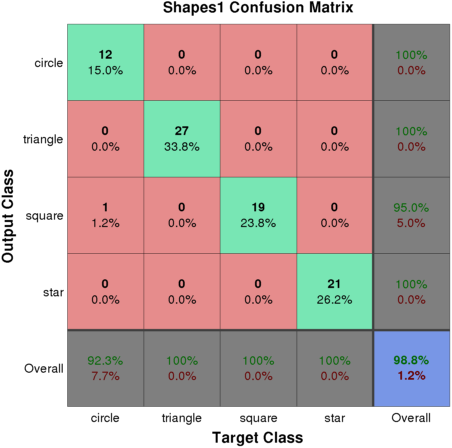
\includegraphics[width=0.3\textwidth]{confusion_matrix_Shapes1}
\caption{No noise}
\end{figure}
\begin{figure}%
\centering
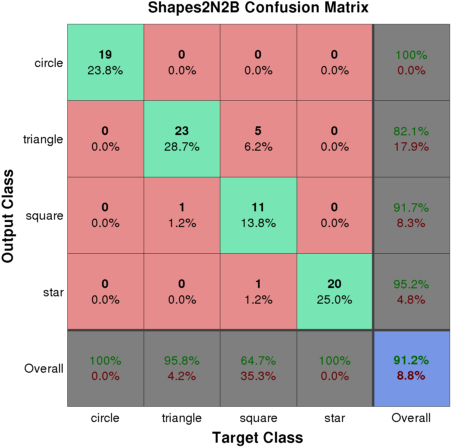
\includegraphics[width=0.3\textwidth]{confusion_matrix_Shapes2N2B}
\caption{Salt and pepper noise}
\end{figure}
\begin{figure}%
\centering
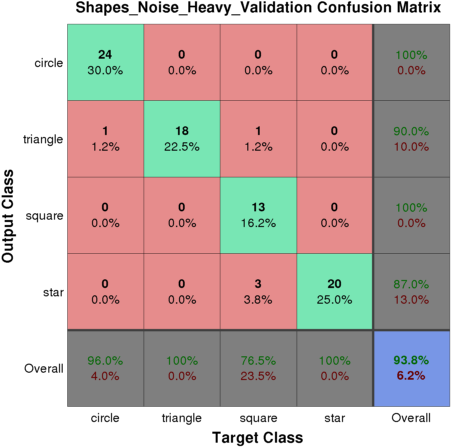
\includegraphics[width=0.3\textwidth]{confusion_matrix_Shapes_Noise_Heavy_Validation}
\caption{Fringes}
\end{figure}
\begin{figure}%
\centering
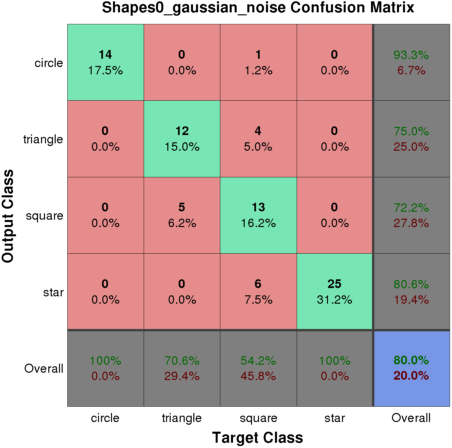
\includegraphics[width=0.3\textwidth]{confusion_matrix_Shapes0_gaussian_noise}
\caption{Gaussian noise}
\end{figure}
\bibliographystyle{IEEEtran}
\bibliography{IEEEabrv,report}
\end{document}

